\documentclass{beamer}
\usepackage{lmodern}
\usepackage{anyfontsize}
\renewcommand{\normalsize}{\fontsize{14}{16}\selectfont}

\usepackage{tikz}

\usepackage{xcolor} % Cargar el paquete para colores

\usepackage{listings}
\lstset{
    language=Haskell,
    basicstyle=\ttfamily,
    % keywordstyle=\color{blue},
    commentstyle=\color{green!40!black},
    stringstyle=\color{orange},
    showstringspaces=false,
    breaklines=true,
    keywordstyle = [3]{\color{blue}},
    morekeywords = [3]{L},
    keywordstyle = [4]{\color{red}},
    morekeywords = [4]{H}
}

\usepackage{tikz}


\usetheme{Madrid}
\usecolortheme{default}

\usepackage{xspace}
\newcommand { \return } {\texttt{return}\xspace}

\newcommand { \vs } {\vspace{0.5cm}}

%Information to be included in the title page:
\title[ROP without Returns] %optional
{Return-Oriented Programming without Returns}

\subtitle{
}

\author[] % (optional, for multiple authors)
{
    Seguridad Informática 
}

\institute[LCC - FCEIA] % (optional)
{
    Facultad de Ciencias Exactas, Ingeniería y Agrimensura\\Universidad Nacional de Rosario
}

\date[Seguridad Informática] % (optional)
{Agosto 2025}

\begin{document}

\frame{
    \titlepage
}

\begin{frame}
    \frametitle{Inyección de Código}
    Una forma de tomar el control de un proceso es: aprovechar un desbordamiento de arreglo en la pila.\\
    
    Pisar la dirección de retorno y saltar a una parte del código o ejecutar código en la misma pila.\\

    \pause

    \textbf{Contramedidas}:
    \begin{itemize}
        \item<2-> Programación fuertemente tipada y validar longitudes.
        \item<2-> No utilizar funciones de biblioteca y diseñar de forma segura.
        \item<2-> Minimizar los puntos de error, capacitar al personal (y tenerlo).
        \item<2-> Verificar los retornos.
        \item<2-> \only<2-2>{Colocar la pila como no ejecutable y agregar canarios.} \only<3->{\textcolor{blue}{Colocar la pila como no ejecutable y agregar canarios.}}
    \end{itemize}
\end{frame}

\begin{frame}
    \frametitle{Programación orientada a los retornos\footnote{\textit{Return-Oriented Programing}}}
    Permite explotar errores de memoria sin inyectar código. \\
    
    Aprovechando la instrucción \return pues realizan un salto y cambia el estado del procesador.\\
    
    \pause
    
    \textbf{Contramedidas}:
    \begin{itemize}
        \item<2-> Revisar los flujos de instrucciones con retornos frecuentes. 
        \item<2-> Validar el invariante de \textit{last-in}, \textit{first-out}.
        \item<2-> No usar la instrucción \return.
    \end{itemize}
\end{frame}

\begin{frame}
    \frametitle{conjunto de \textit{Gadget}}
    \begin{block}{Definición}
        Secuencia de instrucciones que {\only<2->{\color{blue}}ya están presentes en el proceso}, en particular tienen permisos de ejecución. El stack es usado como lugar para almacenar el ``código''.
    \end{block}

    En la programación orientada a los retornos suelen finalizar con la instrucción \return.\vs

    Permiten definir una máquina virtual.\vs
    
    \pause
    
    Se puede buscar posibles \textit{Gadget} mediante algoritmos.

\end{frame}

\begin{frame}
    \frametitle{Convención de llamada}
    \only<1>{
        \begin{figure}[h]
            \centering
            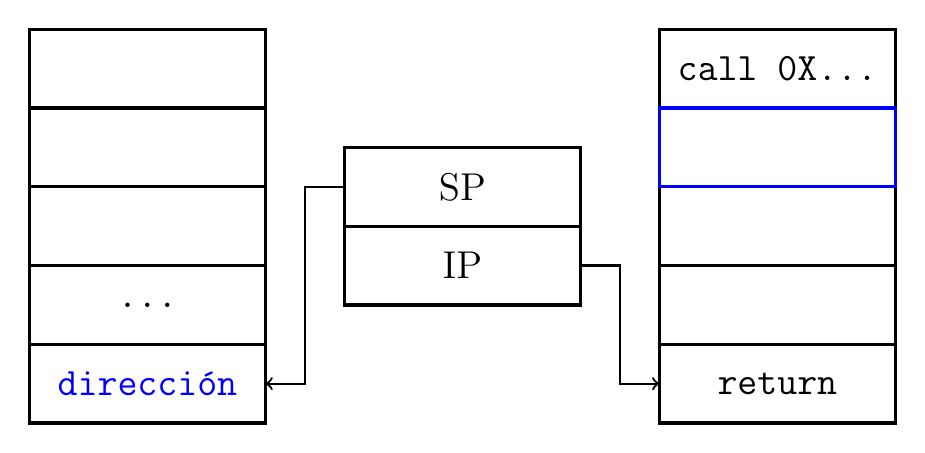
\begin{tikzpicture}
                %% stack
                \draw[black, very thick] (0,0) rectangle (3,1);
                \draw[black, very thick] (0,1) rectangle (3,2);
                \draw[black, very thick] (0,2) rectangle (3,3);
                \draw[black, very thick] (0,3) rectangle (3,4);
                \draw[black, very thick] (0,4) rectangle (3,5);

                \node at (1.5,1.5) {\texttt{...}};
                \node at (1.5,0.5) {\textcolor{blue}{\texttt{dirección}}};

                
                %SP
                \draw[black, very thick] (4,2.5) rectangle (7,3.5);
                \node at (5.5,3) {SP};
                \draw[->, thick] (4,3) -- (3.5,3) |- (3,0.5);

                %IP
                \draw[black, very thick] (4,1.5) rectangle (7,2.5);
                \node at (5.5,2) {IP};
                \draw[->, thick] (7,2) -- (7.5,2) |- (8,0.5);


                %% Código

                \draw[black, very thick] (8,0) rectangle (11,1);
                \draw[black, very thick] (8,1) rectangle (11,2);
                \draw[black, very thick] (8,2) rectangle (11,3);
                \draw[black, very thick] (8,4) rectangle (11,5);
                \draw[blue , very thick] (8,3) rectangle (11,4);

                \node at (9.5,0.5) {\return};
                \node at (9.5,4.5) {\texttt{call 0X...}};


            \end{tikzpicture}
            \caption{Estado de los registro para la pila e instrucciones antes de un \return.}
        \end{figure}

    }
    \pause
    \only<2>{
        \begin{figure}[h]
            \centering
            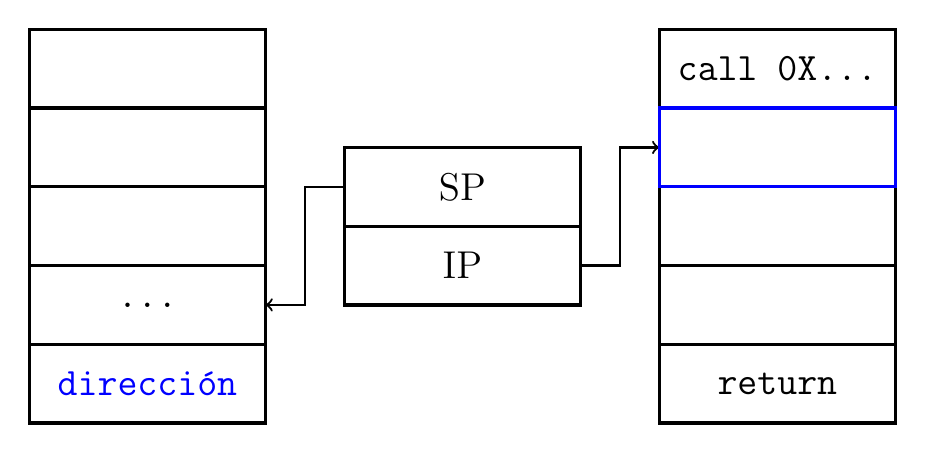
\begin{tikzpicture}
                %% stack
                \draw[black, very thick] (0,0) rectangle (3,1);
                \draw[black, very thick] (0,1) rectangle (3,2);
                \draw[black, very thick] (0,2) rectangle (3,3);
                \draw[black, very thick] (0,3) rectangle (3,4);
                \draw[black, very thick] (0,4) rectangle (3,5);

                \node at (1.5,1.5) {\texttt{...}};
                \node at (1.5,0.5) {\textcolor{blue}{\texttt{dirección}}};

                
                %SP
                \draw[black, very thick] (4,2.5) rectangle (7,3.5);
                \node at (5.5,3) {SP};
                \draw[->, thick] (4,3) -- (3.5,3) |- (3,1.5);

                %IP
                \draw[black, very thick] (4,1.5) rectangle (7,2.5);
                \node at (5.5,2) {IP};
                \draw[->, thick] (7,2) -- (7.5,2) |- (8,3.5);


                %% Código

                \draw[black, very thick] (8,0) rectangle (11,1);
                \draw[black, very thick] (8,1) rectangle (11,2);
                \draw[black, very thick] (8,2) rectangle (11,3);
                \draw[black, very thick] (8,4) rectangle (11,5);
                \draw[blue , very thick] (8,3) rectangle (11,4);

                \node at (9.5,0.5) {\return};
                \node at (9.5,4.5) {\texttt{call 0X...}};


            \end{tikzpicture}
            \caption{Estado de los registro para la pila e instrucciones después de un \return.}
        \end{figure}
    }
\end{frame}

\begin{frame}
    \frametitle{Programación orientada a los retornos sin retornos\footnote{\textit{Return-Oriented Programing without Returns}}}
    \textbf{Se asume}:
    \begin{itemize}
        \item Puede haber implementado un modelo de lectura o ejecución exclusivos ($W \oplus X$).
        \item Puede haber contramedidas para la programación orientada a los retornos.
        \item Hay una aplicación vulnerable a los ataques.
    \end{itemize}

    Necesitamos otras formas de tener las 2 propiedades del \return:
    \begin{enumerate}
        \item Trasferir el control de ejecución con un salto indirecto.
        \item Actualizar el estado del proceso (no volver a la misma instrucción)
    \end{enumerate}
\end{frame}

\begin{frame}
    \frametitle{Si no usamos \return}
    \only<1>{
        \begin{figure}[h]
            \centering
            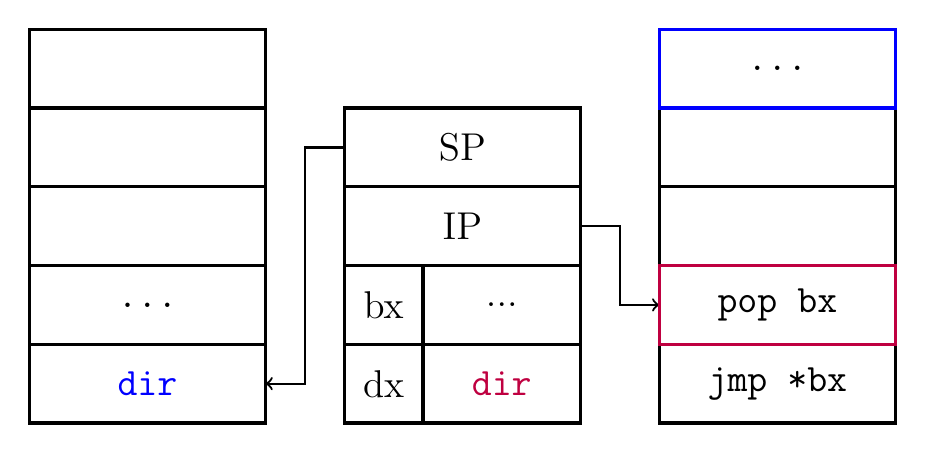
\begin{tikzpicture}
                %% stack
                \draw[black, very thick] (0,0) rectangle (3,1);
                \draw[black, very thick] (0,1) rectangle (3,2);
                \draw[black, very thick] (0,2) rectangle (3,3);
                \draw[black, very thick] (0,3) rectangle (3,4);
                \draw[black, very thick] (0,4) rectangle (3,5);

                \node at (1.5,1.5) {\texttt{...}};
                \node at (1.5,0.5) {\textcolor{blue}{\texttt{dir}}};

                
                %SP
                \draw[black, very thick] (4,3) rectangle (7,4);
                \node at (5.5,3.5) {SP};
                \draw[->, thick] (4,3.5) -- (3.5,3.5) |- (3,0.5);

                %IP
                \draw[black, very thick] (4,2) rectangle (7,3);
                \node at (5.5,2.5) {IP};
                \draw[->, thick] (7,2.5) -- (7.5,2.5) |- (8,1.5);

                %BX
                \draw[black, very thick] (4,1) rectangle (5,2);
                \draw[black, very thick] (5,1) rectangle (7,2);
                \node at (4.5,1.5) {bx};
                \node at (6,1.5)   {...};

                %DX
                \draw[black, very thick] (4,0) rectangle (5,1);
                \draw[black, very thick] (5,0) rectangle (7,1);
                \node at (4.5,0.5) {dx};
                \node at (6,0.5)   {\textcolor{purple}{\texttt{dir}}};

                
                %% Código

                \draw[black, very thick] (8,0) rectangle (11,1);
                \draw[black, very thick] (8,2) rectangle (11,3);
                \draw[black, very thick] (8,3) rectangle (11,4);
                \draw[blue , very thick] (8,4) rectangle (11,5);
                \draw[purple, very thick] (8,1) rectangle (11,2);
                
                \node at (9.5,1.5) {\texttt{pop bx}};
                \node at (9.5,0.5) {\texttt{jmp *bx}};
                \node at (9.5,4.5) {\texttt{...}};

            \end{tikzpicture}
            \caption{Ejecución del ``trampolín'': \texttt{pop} saca de la pila y coloca en \textbf{bx}}
        \end{figure}

    }
    \pause
    \only<2>{
        \begin{figure}[h]
            \centering
            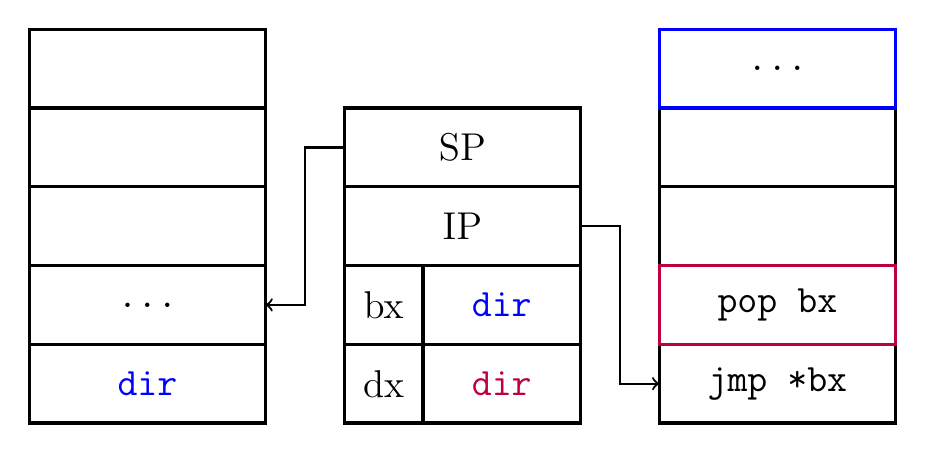
\begin{tikzpicture}
                %% stack
                \draw[black, very thick] (0,0) rectangle (3,1);
                \draw[black, very thick] (0,1) rectangle (3,2);
                \draw[black, very thick] (0,2) rectangle (3,3);
                \draw[black, very thick] (0,3) rectangle (3,4);
                \draw[black, very thick] (0,4) rectangle (3,5);

                \node at (1.5,1.5) {\texttt{...}};
                \node at (1.5,0.5) {\textcolor{blue}{\texttt{dir}}};

                
                %SP
                \draw[black, very thick] (4,3) rectangle (7,4);
                \node at (5.5,3.5) {SP};
                \draw[->, thick] (4,3.5) -- (3.5,3.5) |- (3,1.5);

                %IP
                \draw[black, very thick] (4,2) rectangle (7,3);
                \node at (5.5,2.5) {IP};
                \draw[->, thick] (7,2.5) -- (7.5,2.5) |- (8,0.5);

                %BX
                \draw[black, very thick] (4,1) rectangle (5,2);
                \draw[black, very thick] (5,1) rectangle (7,2);
                \node at (4.5,1.5) {bx};
                \node at (6,1.5)   {\textcolor{blue}{\texttt{dir}}};

                %DX
                \draw[black, very thick] (4,0) rectangle (5,1);
                \draw[black, very thick] (5,0) rectangle (7,1);
                \node at (4.5,0.5) {dx};
                \node at (6,0.5)   {\textcolor{purple}{\texttt{dir}}};

                
                %% Código

                \draw[black, very thick] (8,0) rectangle (11,1);
                \draw[black, very thick] (8,2) rectangle (11,3);
                \draw[black, very thick] (8,3) rectangle (11,4);
                \draw[blue , very thick] (8,4) rectangle (11,5);
                \draw[purple, very thick] (8,1) rectangle (11,2);
                
                \node at (9.5,1.5) {\texttt{pop bx}};
                \node at (9.5,0.5) {\texttt{jmp *bx}};
                \node at (9.5,4.5) {\texttt{...}};

            \end{tikzpicture}
            \caption{Ejecución del ``trampolín'': \texttt{jmp} salta a la dirección de \textbf{bx}}
        \end{figure}

    }
    \pause
    \only<3>{
        \begin{figure}[h]
            \centering
            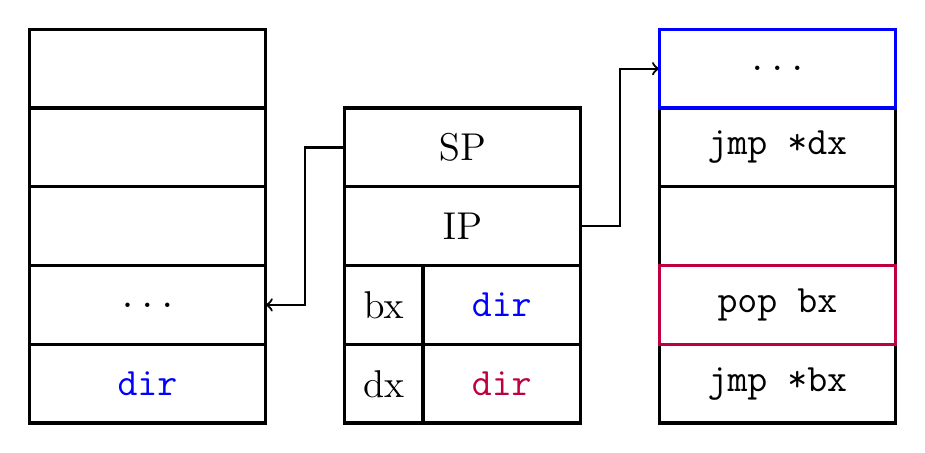
\begin{tikzpicture}
                %% stack
                \draw[black, very thick] (0,0) rectangle (3,1);
                \draw[black, very thick] (0,1) rectangle (3,2);
                \draw[black, very thick] (0,2) rectangle (3,3);
                \draw[black, very thick] (0,3) rectangle (3,4);
                \draw[black, very thick] (0,4) rectangle (3,5);

                \node at (1.5,1.5) {\texttt{...}};
                \node at (1.5,0.5) {\textcolor{blue}{\texttt{dir}}};

                
                %SP
                \draw[black, very thick] (4,3) rectangle (7,4);
                \node at (5.5,3.5) {SP};
                \draw[->, thick] (4,3.5) -- (3.5,3.5) |- (3,1.5);

                %IP
                \draw[black, very thick] (4,2) rectangle (7,3);
                \node at (5.5,2.5) {IP};
                \draw[->, thick] (7,2.5) -- (7.5,2.5) |- (8,4.5);

                %BX
                \draw[black, very thick] (4,1) rectangle (5,2);
                \draw[black, very thick] (5,1) rectangle (7,2);
                \node at (4.5,1.5) {bx};
                \node at (6,1.5)   {\textcolor{blue}{\texttt{dir}}};

                %DX
                \draw[black, very thick] (4,0) rectangle (5,1);
                \draw[black, very thick] (5,0) rectangle (7,1);
                \node at (4.5,0.5) {dx};
                \node at (6,0.5)   {\textcolor{purple}{\texttt{dir}}};

                
                %% Código

                \draw[black, very thick] (8,0) rectangle (11,1);
                \draw[black, very thick] (8,2) rectangle (11,3);
                \draw[black, very thick] (8,3) rectangle (11,4);
                \draw[blue , very thick] (8,4) rectangle (11,5);
                \draw[purple, very thick] (8,1) rectangle (11,2);
                
                \node at (9.5,1.5) {\texttt{pop bx}};
                \node at (9.5,0.5) {\texttt{jmp *bx}};
                \node at (9.5,4.5) {\texttt{...}};
                \node at (9.5,3.5) {\texttt{jmp *dx}};

            \end{tikzpicture}
            \caption{Ejecución del código del \textit{gadget}. Debe terminar con un salto al trampolín.}
        \end{figure}

    }
\end{frame}

\begin{frame}
    \frametitle{INTEL x86}
    En este caso el conjunto de \textit{gadgets} proviene de \textbf{libc} y \textbf{libxul}. \\
    
    Que el compilador evite su aparición es complicado.\vs

    Los \textit{gadgets} son 19: \texttt{load} (\texttt{immediate}), \texttt{move}, \texttt{store}, \texttt{add} (\texttt{immediate}), \texttt{subtract}, \texttt{negate}, \texttt{and} (\texttt{immediate}), \texttt{or} (\texttt{immediate}), \texttt{xor} (\texttt{immediate}), \textit{complement}, \texttt{branch unconditional}, \texttt{branch conditional}, \texttt{set less than} y \texttt{call}. 
\end{frame}

\begin{frame}
    \frametitle{INTEL x86 (observaciones)}
    \begin{itemize}
        % \item 
        \item Se busca que las operaciones actualicen valores en memoria.
        \item  Las interacciones con memoria requieren registros intermedios, porque se usan 2 niveles de indirección.
        \item Las ramas condicionales actualizan valores de memoria y no el registro de instrucciones.
        \item La convención para hacer llamadas a funciones utilizada en el paper no es la actual en Linux.
    \end{itemize}
\end{frame}

\begin{frame}
    \frametitle{INTEL x86 (\textit{gadget})}
    \begin{figure}
        \centering
        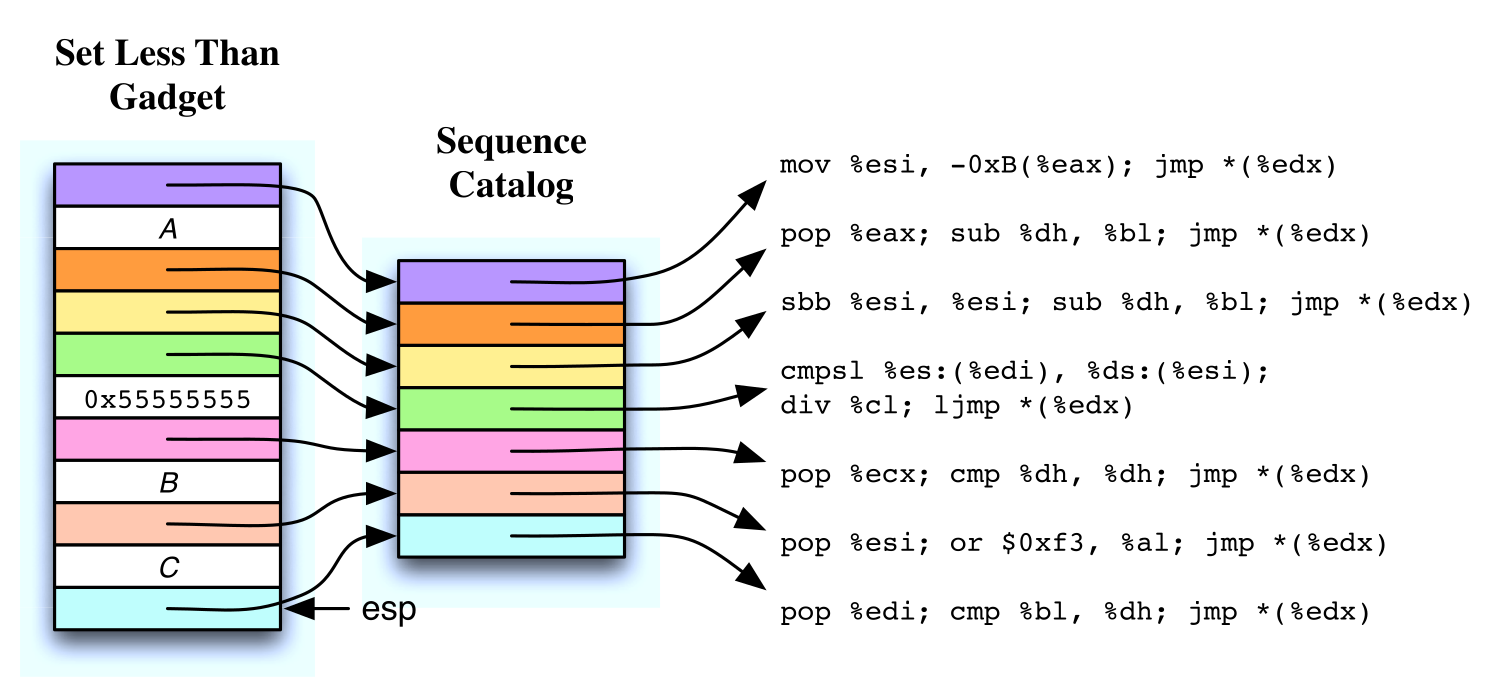
\includegraphics[scale=0.2]{gadgetx86.png}
    \end{figure}
\end{frame}

\begin{frame}
    \frametitle{ARM}

    En ARM no tenemos algo como la convención de llamada en x86. El epílogo no funciona igual, hay 16 registros los cuales se pueden modificar directamente (incluido el de instrucciones).

    \vs

    La instrucción \texttt{bl} y \texttt{blx} son la que nos permiten los saltos pero solo \texttt{blx} permite saltar con direcciones en registros. Desde donde se salta se almacena en r14 (lr). 

\end{frame}

\begin{frame}
    \frametitle{ARM}
    \begin{columns}
        \column{0.6\textwidth}
            \begin{figure}
            \centering
                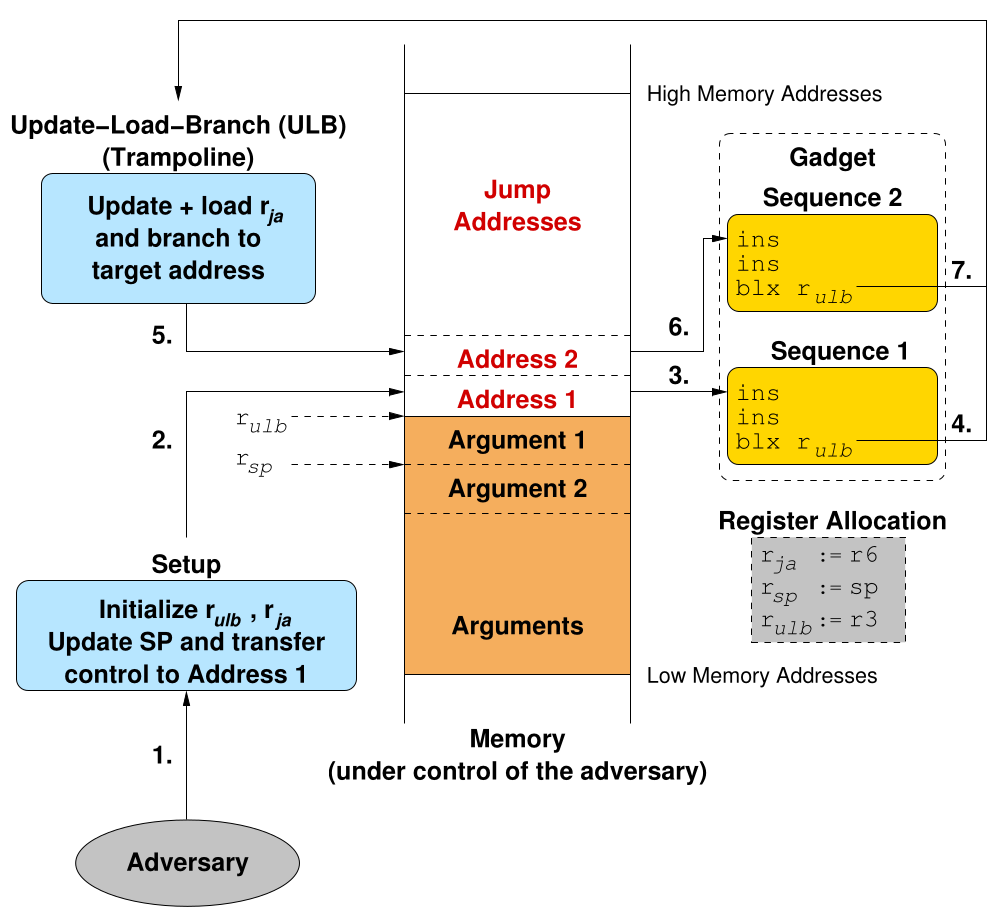
\includegraphics[scale=0.2]{ideaARM.png}
            \end{figure}
        \column{0.4\textwidth}
        \only<1>{
            \begin{center}
                ULB
            \end{center}
            
            \texttt{adds} r6, \#4;\\
            \texttt{ldr} r5, [r6, \#124];\\
            \texttt{blx} r5;\\
        }
        \pause
        \only<2>{
            \begin{center}
                \textcolor{blue}{Update }\textcolor{purple}{Load }\textcolor{brown}{Branch}
            \end{center}
            
            \textcolor{blue}{\texttt{adds} r6, \#4;}\\
            \textcolor{purple}{\texttt{ldr} r5, [r6, \#124];}\\
            \textcolor{brown}{\texttt{blx} r5;}\\
        }
    \end{columns}
\end{frame}

\begin{frame}
    \frametitle{ARM (observaciones)}
    \begin{itemize}
        \item Las instrucciones deben terminar con \texttt{blx}.
        \item Se construyeron los \textit{gargets} con \textbf{libc} y \textbf{libwebcore}
        \item Se requieren 3 registros en lugar de 1.
        \item Por limitaciones de la arquitectura hacen que manejar memoria sea más complejo.
        \item La forma de realizar operaciones aritmético-lógicas es idéntica, igualmente los condicionales.
        \item Este ataque no puede ser detectado por \textit{validadores de direcciones de retorno}\footnote{return address checker}. No se modifica la pila.
    \end{itemize}
    
\end{frame}

\begin{frame}
    \frametitle{ARM (\textit{gadget})}
    \begin{figure}
        \centering
        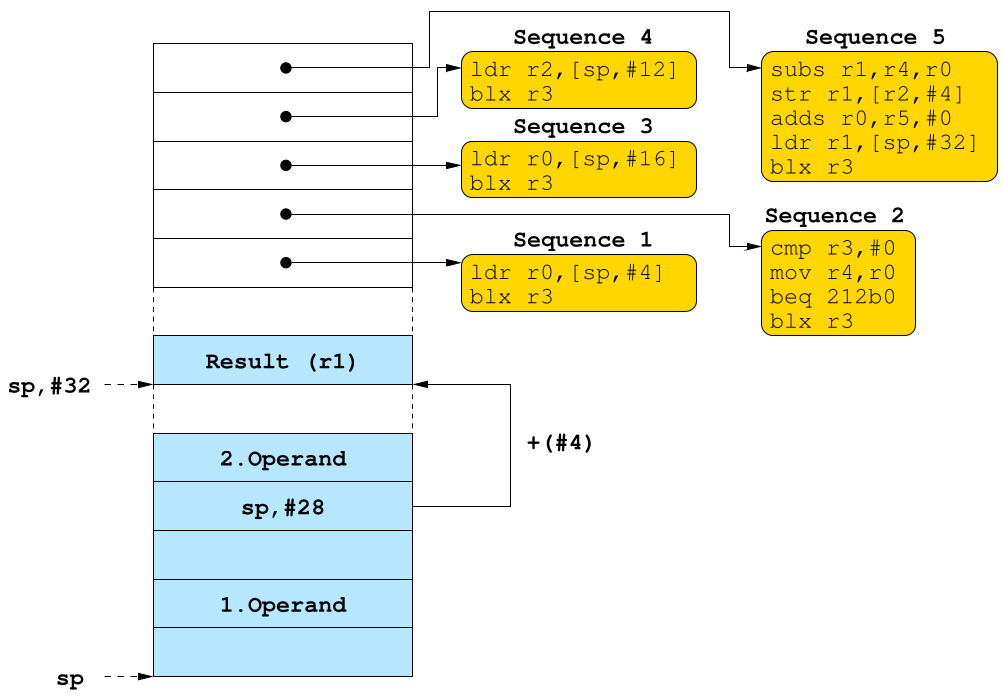
\includegraphics[scale=0.3]{gadgetARM.png}
    \end{figure}
\end{frame}

\begin{frame}
    \frametitle{Ataques Concretos}
    \only<1>{
        \textbf{Linux Intel x86}
        \begin{columns}
        \column{0.5\textwidth}
        \begin{figure}
            \centering
            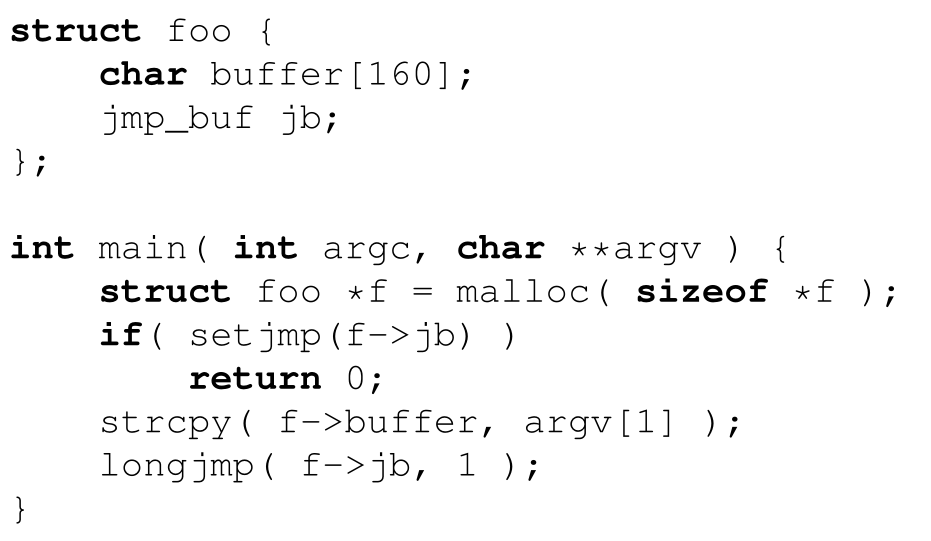
\includegraphics[scale=0.15]{LinuxIntel86.png}
        \end{figure}
        \column{0.5\textwidth}
            Se dá un \textit{shellcode egg} a este programa con: 
            \begin{itemize}
                \item El programa (ROPWR).
                \item Los datos (programa a ejecutar).
                \item el catálogo de instrucciones (doble indirección).
                \item Datos para pisar \texttt{foo}.
            \end{itemize}
        \end{columns}
    }
    \pause
    \only<2>{
        \textbf{Google Android ARM}
        \begin{columns}
        \column{0.5\textwidth}
        \begin{figure}
            \centering
            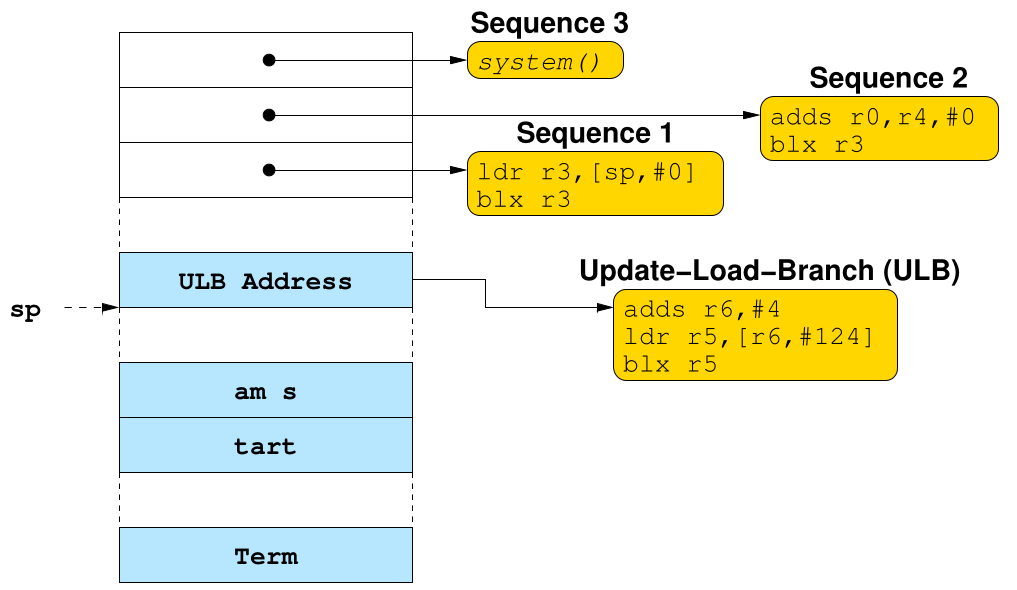
\includegraphics[scale=0.15]{GoogleAndroidARM.png}
        \end{figure}
        \column{0.5\textwidth}
            Obtener una shell en el emulador para el desarrollador de android.\\
            Se utiliza el mismo código que antes a traves de una interfaz de java para C.
        \end{columns}
    }
\end{frame}

\begin{frame}
    \frametitle{Conclusiones}
    \begin{itemize}
        \item Encontrar un trampolín basta para construir a su alrededor un conjunto de \textit{gargets}.
        \item Esta nueva forma de programar es un problema grave de seguridad.
        \item Las posibles mitigaciones pueden tener una gran penalidad.
    \end{itemize}
\end{frame}


\end{document}